\chapter{Materiais e Métodos}

A prova de conceito será feita a partir de uma placa receptora e outra transmissora fabricadas utilizando a infraestrutura disponível no Laboratório de Microeletrônica da USP (LME). A estrutura da solução proposta é mostrado no diagrama de bloco da Figura \ref{blocos}. As entradas e saídas externas do sistema são:
\begin{itemize}
    \item Oscilador local: Fornecerá um sinal de frequência entre 16,3 GHz e 18,3 GHz que será utilizado para gerar a onda portadora de 60 GHz para o envio dos dados;
    \item FPGA: Modulação/demodulação do sinal de vídeo no formato I/Q entre o computador e o sistema de transmissão/recepção;
    \item FRDM-KL25Z: Interface de comunicação serial/SPI entre o computador e o sistema transmissor/receptor utilizado para configuração.
\end{itemize}

\begin{figure}[ht]
\centering
%\captionsetup{justification=centering}
\caption{Diagrama de blocos - transmissor/receptor}
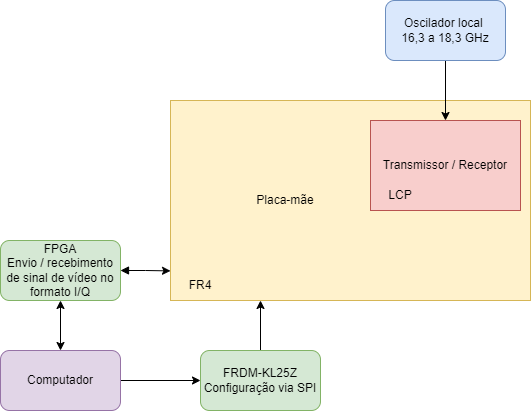
\includegraphics[width = \linewidth - 3cm]{Estrutura.drawio.png}

\source{De autoria própria}
\centering
\label{blocos}
\end{figure}

O sistema transmissor/receptor é composto por duas placas de circuito impresso, \textit{Printed Circuit Boards (PCB)}, a placa-mãe e a placa-filha. A placa-mãe será responsável por receber e enviar os sinais para os componentes externos e regular as tensões de alimentação necessárias para a placa-filha. A comunicação entre as placas é feita a partir de um conector placa-placa. A placa-filha será responsável por receber o sinal do oscilador local, modular o sinal de entrada recebido pela placa-mãe e enviar/receber os dados em 60 GHz, utilizando os circuitos integrados HMC6300 e HMC6301 para o transmissor e receptor, respectivamente. A antena utilizada será fabricada na própria placa-filha.

\section{Fabricação das PCBs}

As placas de circuito impresso são desenhadas em \textit{software}s como Altium Designer e KiCAD. O processo de fabricação das PCBs será feito por uma cortadora a \textit{\textit{laser}} mostrada na figura \ref{lpkf}, fabricado pela LPKF, para os furos, isolação das trilhas e criação do \textit{stencil} para solda dos componentes. As rotinas para cada processo são criadas pelo \textit{software} CircuitCAM a partir dos arquivos Gerber gerados pelos \textit{software} de \textit{Electronic Computer-Aided Design (ECAD)}. A sequência dos processos é mostrada a seguir:

 \begin{figure}[htbp]
    \centering
    %\captionsetup{justification=centering}
    \caption{Cortadora a \textit{laser}}
    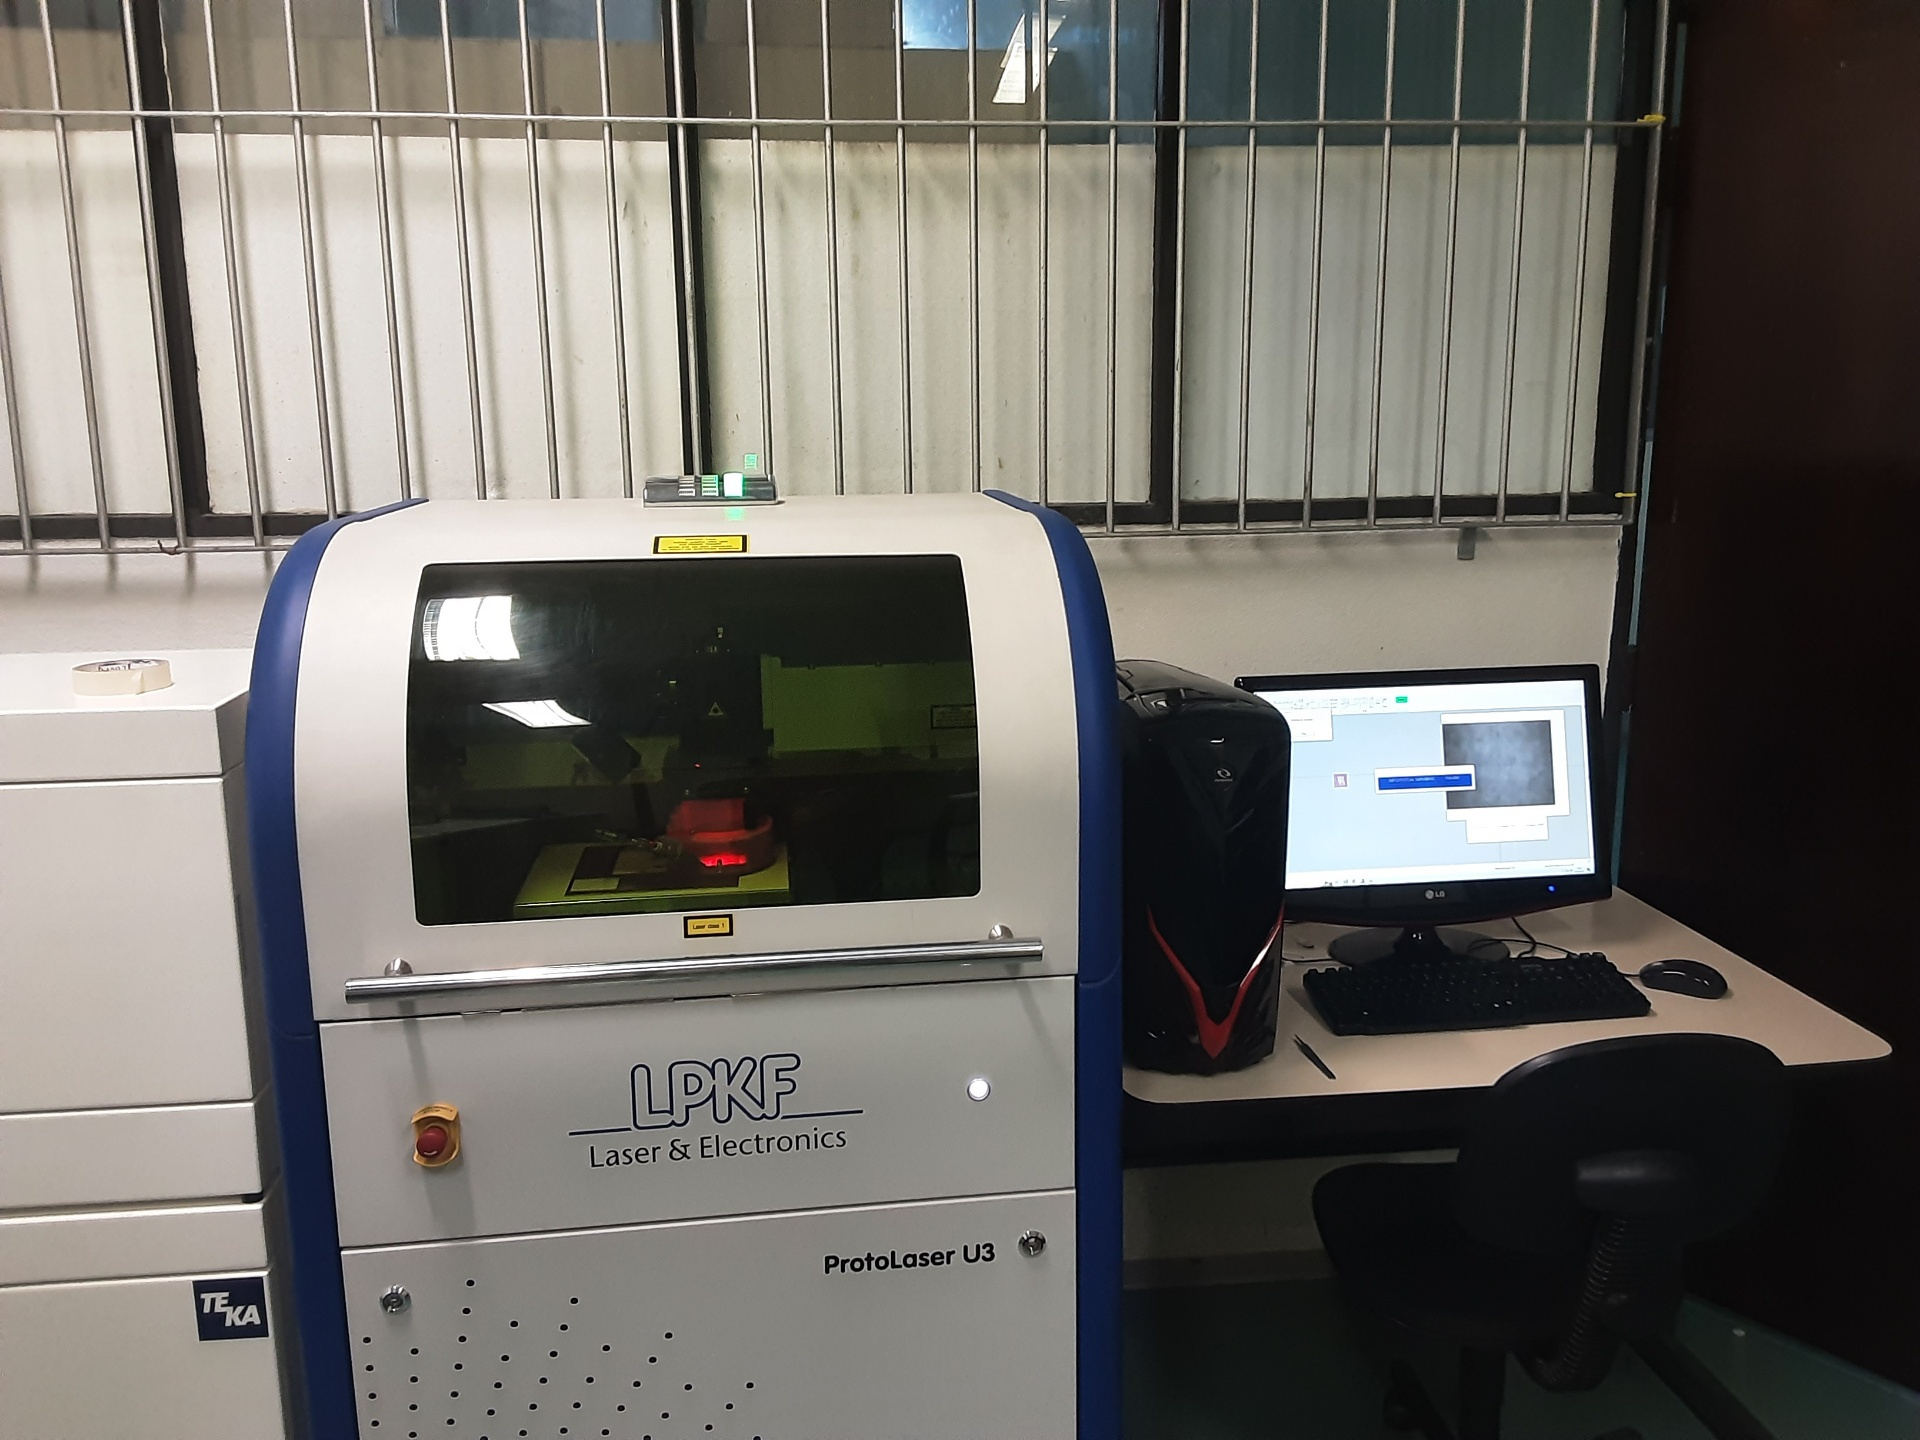
\includegraphics[width = \linewidth - 5cm]{lpkf.jpg}
    
    \source{De autoria própria}
    \centering
    \label{lpkf}
\end{figure}

\begin{enumerate}
    \item \textbf{Furação}: Os furos são feitos pelo corte a \textit{laser} em múltiplas etapas, alterando a altura do ponto focal para cortar através do material. Nesse processo também são criados os pontos fiduciais para posterior alinhamento;
    
    \item \textbf{Metalização das vias}: As vias, que tem a função de ligar as trilhas eletricamente entre a camada superior e a camada inferior, são metalizadas por meio de deposição \textit{electroless} de cobre por meio de um processo industrial, M-Copper Omega \cite{macdermid}, desenvolvido pela MacDermid, como mostrado na Figura \ref{electroless}.
    
        \begin{figure}[htbp]
            \centering
            %\captionsetup{justification=centering}
            \caption{Deposição \textit{electroless}}
            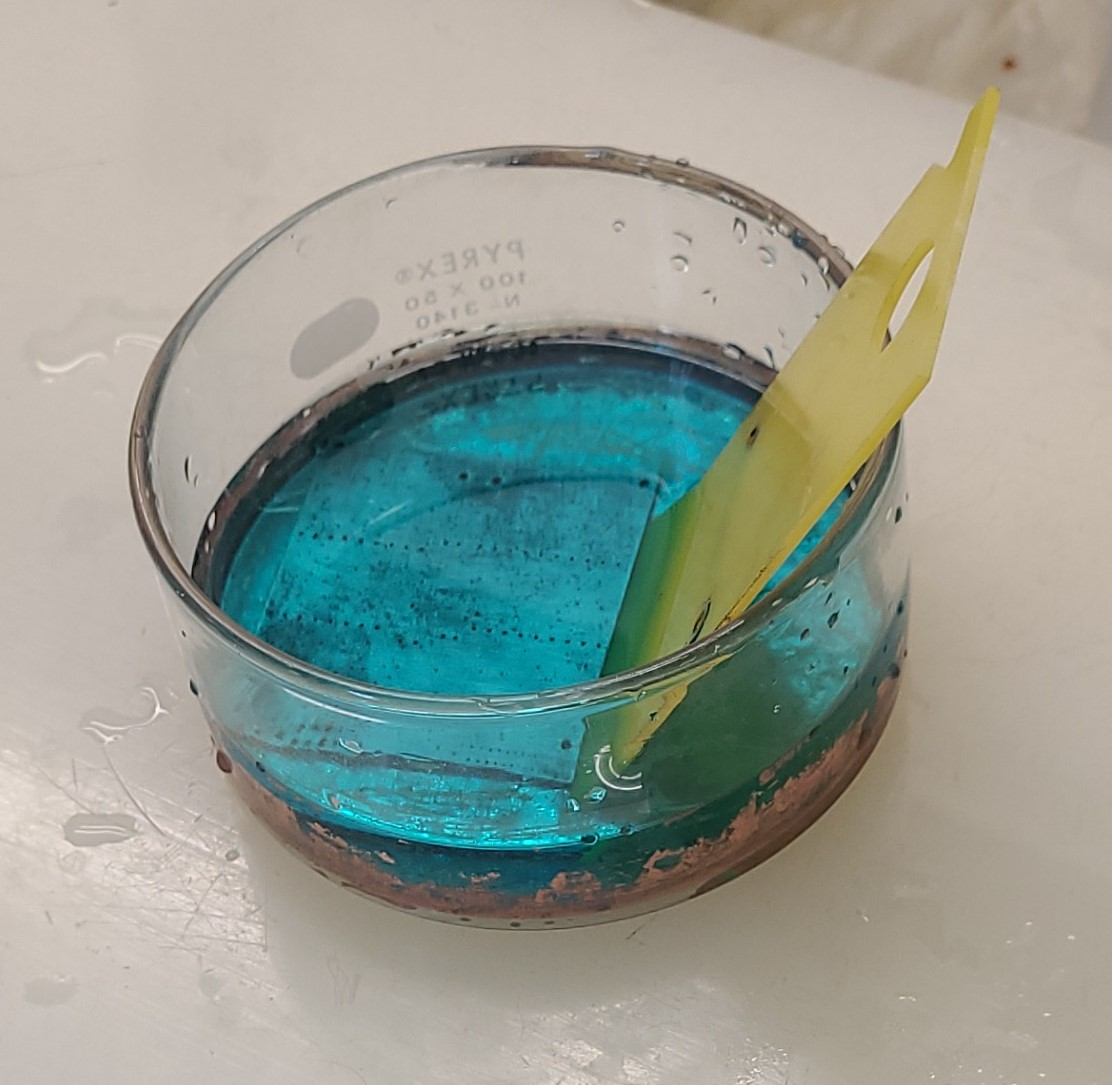
\includegraphics[width = \linewidth - 5cm]{IMG-20220427-WA0010.jpeg}
            
            \source{De autoria própria}
            \centering
            \label{electroless}
        \end{figure}
    Em seguida, é feito uma deposição eletrolítica para aumentar a espessura do cobre na via. Esse processo utiliza uma tensão aplicada no formato \textit{periodic pulse reverse (PPR)} \cite{Zhu_2014}, de forma a aumentar a espessura do cobre apenas nas vias;
    
    \item \textbf{Isolação das trilhas}: Após o processo de metalização, a placa em produção volta ao corte a \textit{laser}. Utilizando os pontos fiduciais para realinhar e referenciar a máquina. Para remover as áreas de cobre indesejadas no \textit{layout} e criar as trilhas de sinais, o processo é dividido em duas etapas, \textit{rubout} e \textit{heat}.
    
    O primeiro separa a região em filetes paralelos, separando termicamente cada linha de cobre, como mostrado na Figura \ref{rubout}. Em seguida, a etapa de \textit{heat} esquenta os filetes, como estão isolados termicamente do restante do cobre da placa, eles esquentam mais e se descolam do substrato, como mostrado na Figura \ref{heat}, sendo facilmente removidos pelo exaustor da máquina \cite{KMETEC20098598}.
    
        \begin{figure}[htbp]
            \centering
            %\captionsetup{justification=centering}
            \caption{Etapa de \textit{rubout}}
            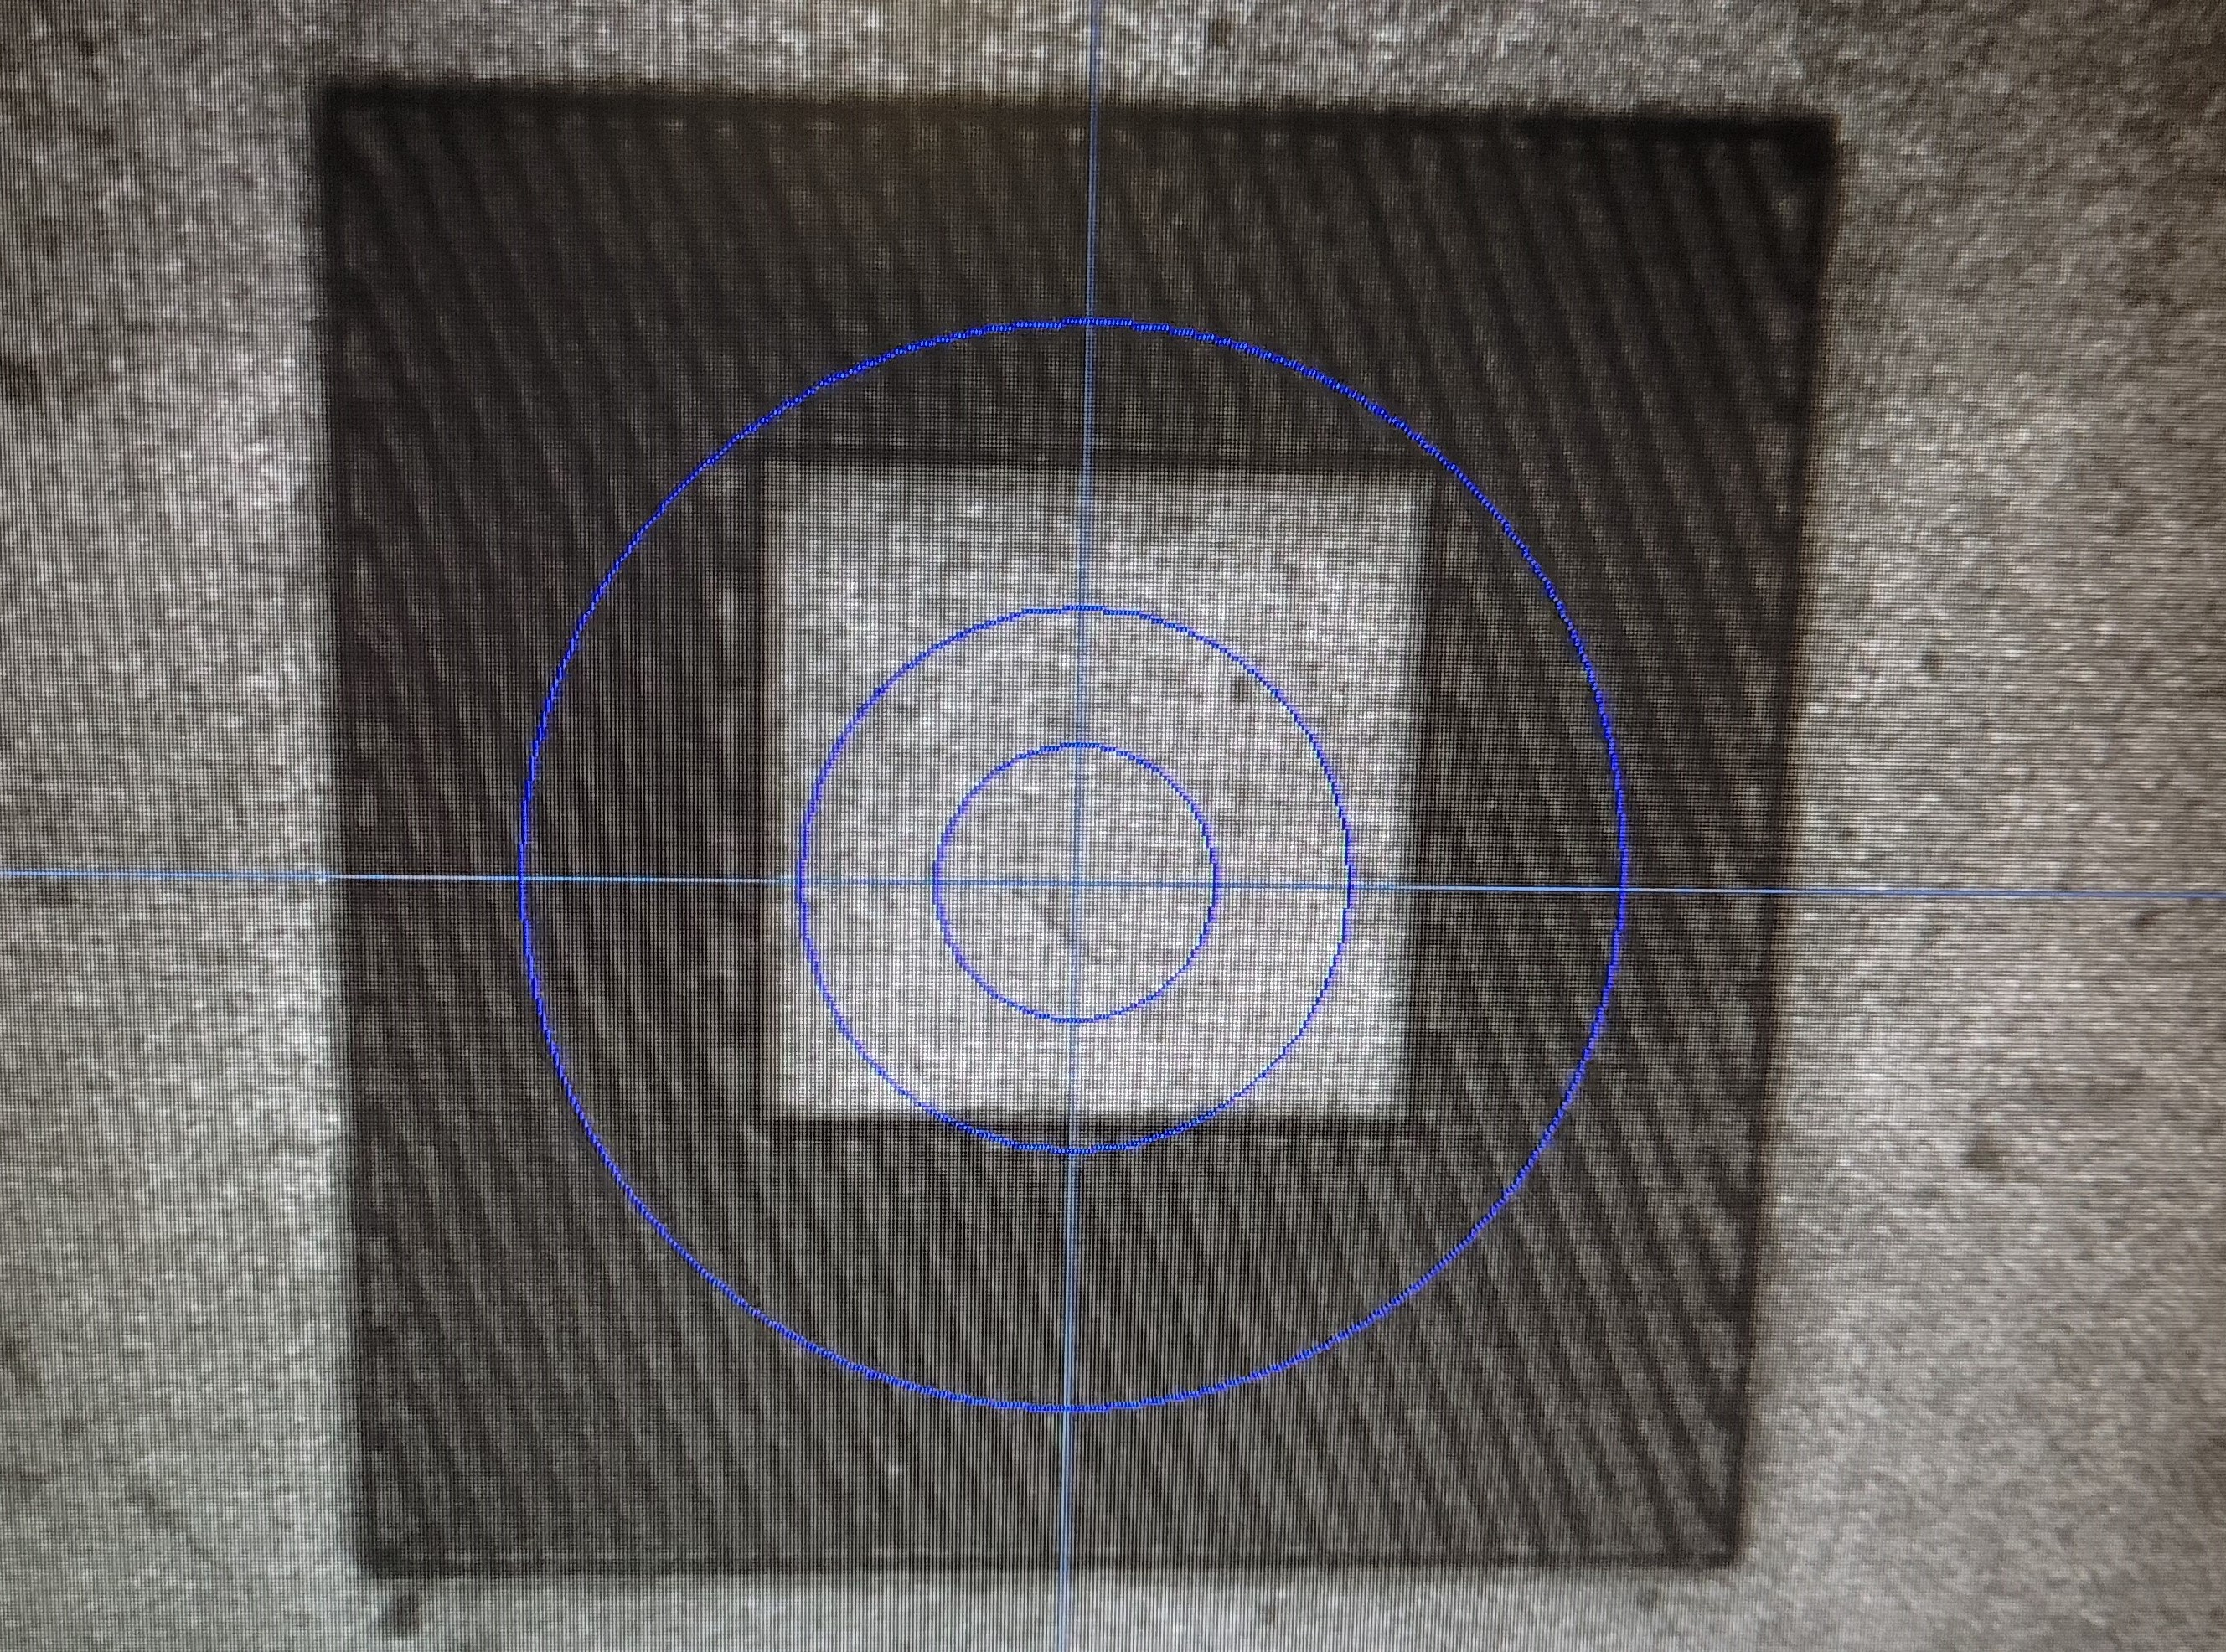
\includegraphics[width = \linewidth - 8cm]{rubout.jpg}
            
            \source{De autoria própria}
            \centering
            \label{rubout}
        \end{figure}
        
        \begin{figure}[htbp]
            \centering
            %\captionsetup{justification=centering}
            \caption{Etapa de \textit{heat}}
            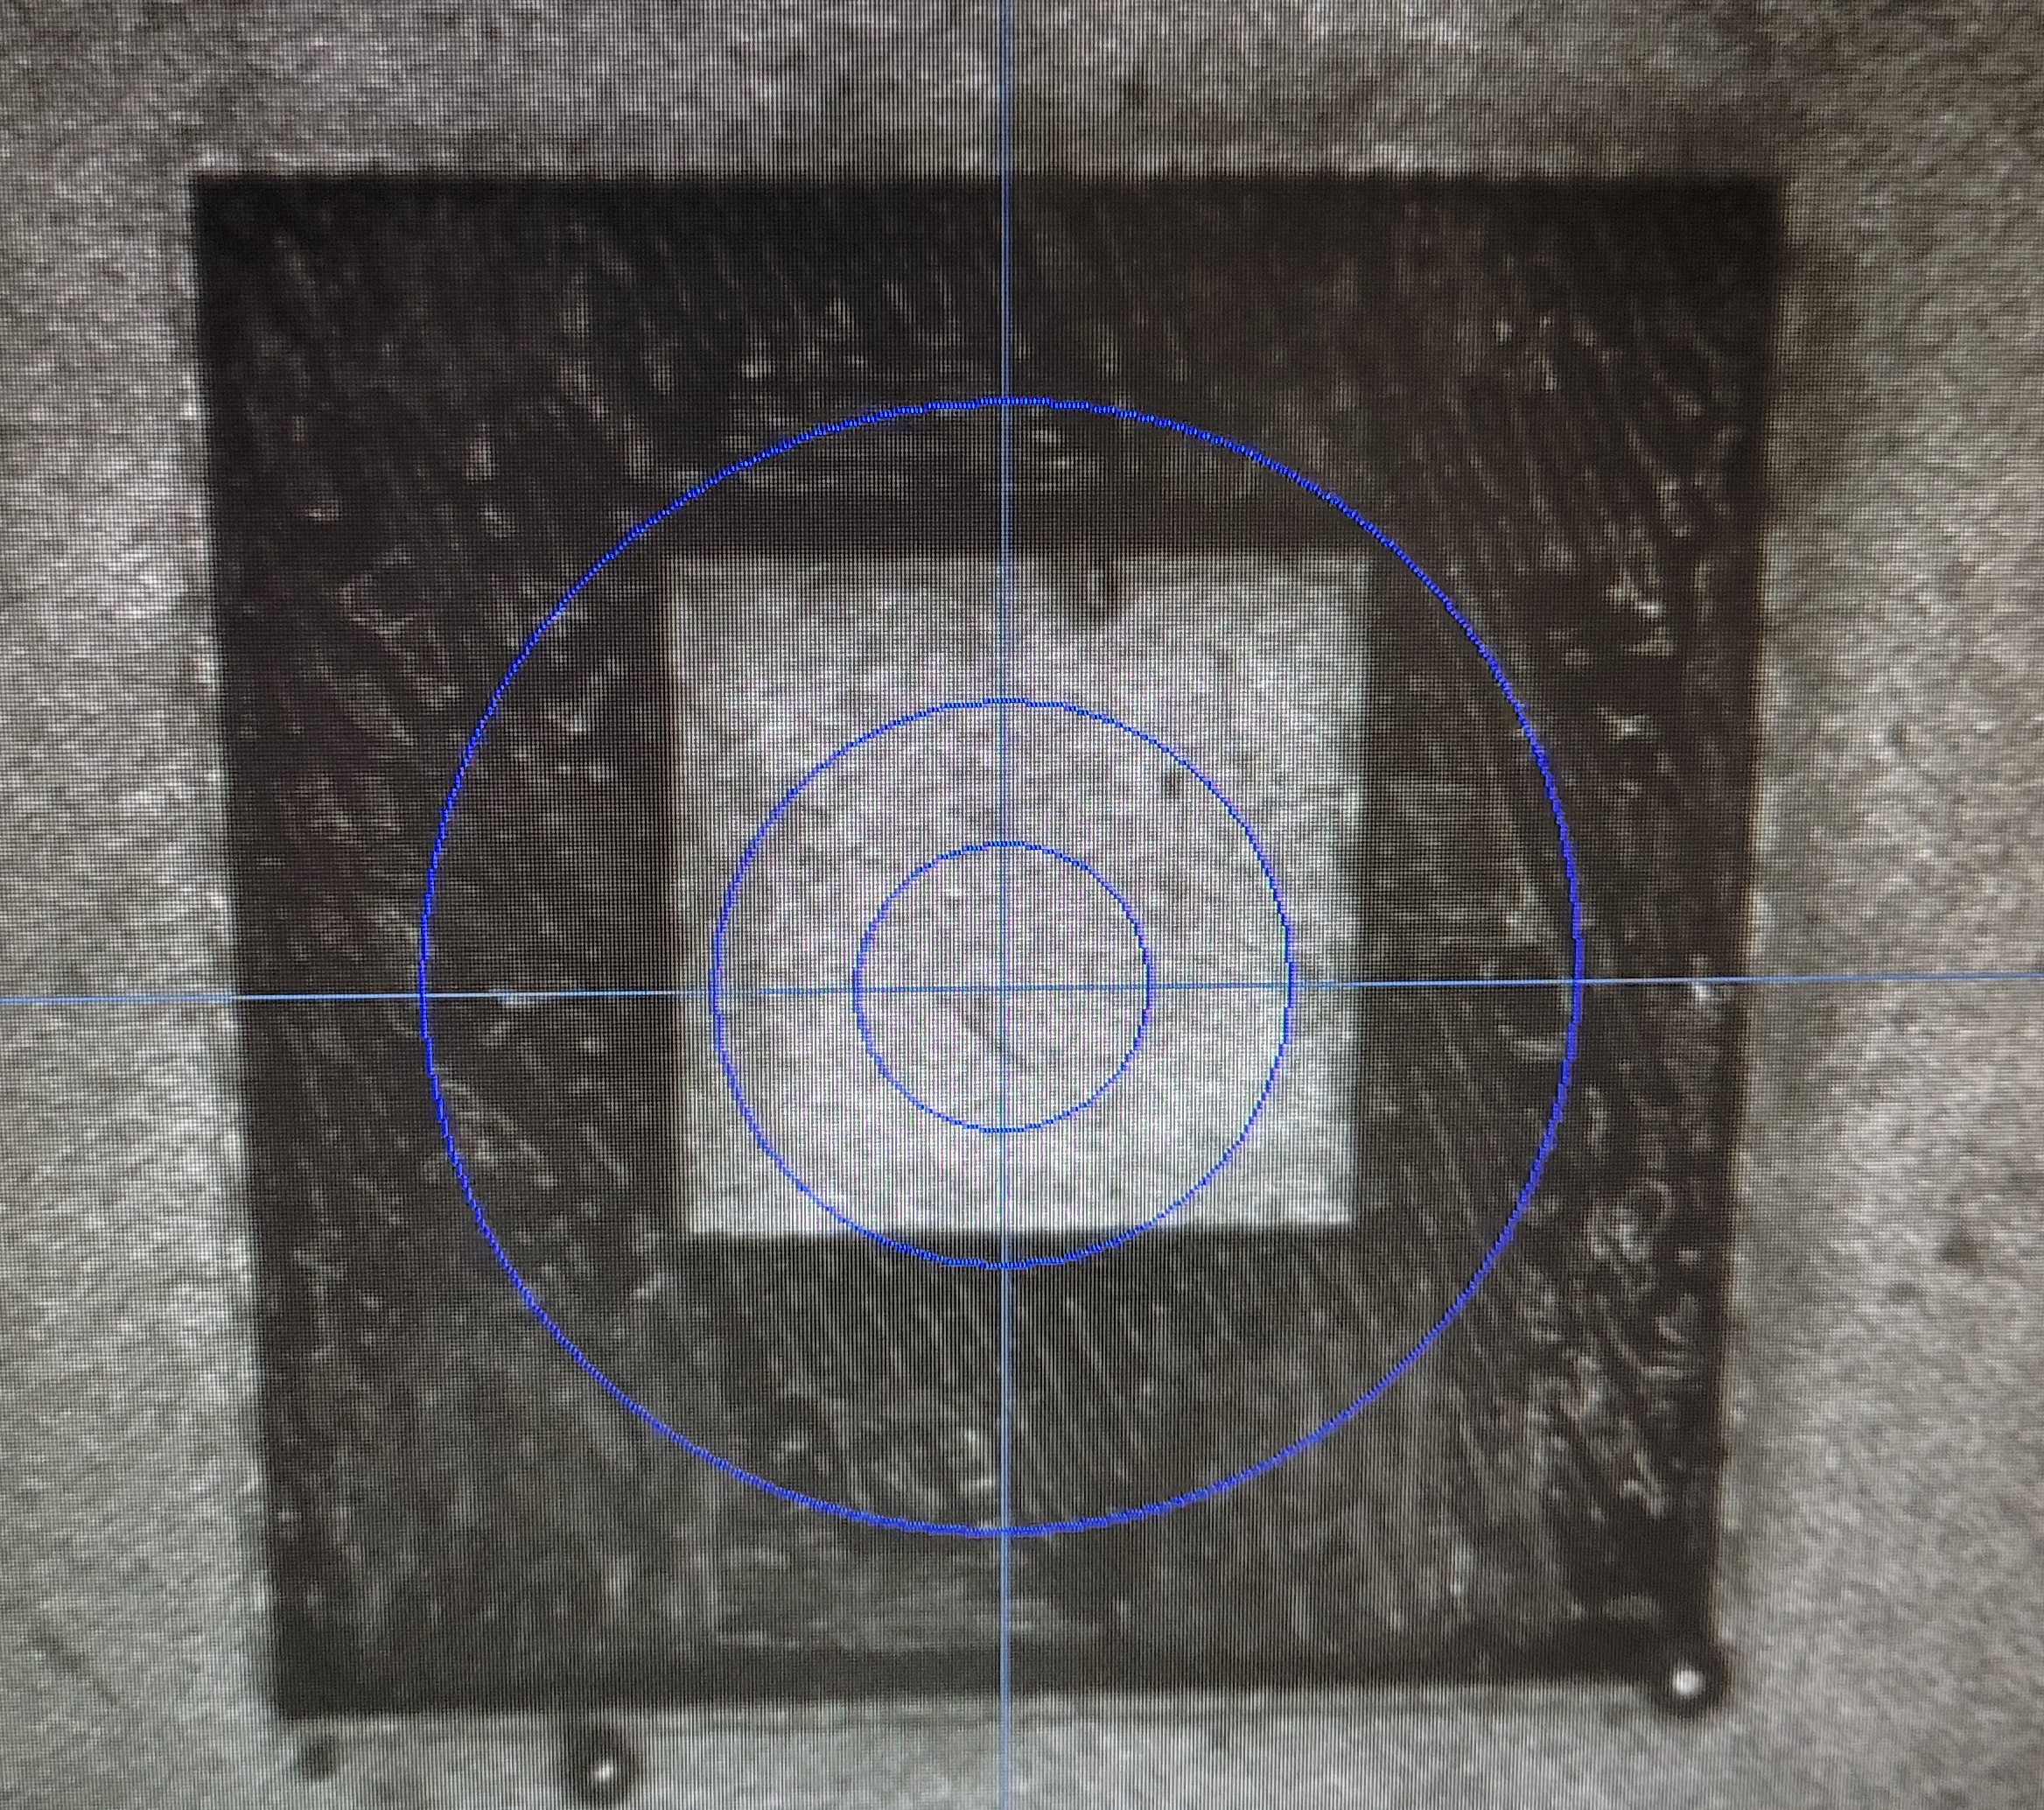
\includegraphics[width = \linewidth - 8cm]{heat.jpg}
            
            \source{De autoria própria}
            \centering
            \label{heat}
        \end{figure}
    
    %\item \textit{\textbf{Stencil}}: Para aplicar a pasta de solda apenas nos lugares corretos, é feito um \textit{stencil}. O material utilizado é um acetato de espessura  $175 \mu m$, no qual foram cortados os contornos dos pontos de aplicação da pasta de solda.
    
    %\item \textbf{Posicionamento e solda dos componentes}: 
\end{enumerate}

Os parâmetro da cortadora a \textit{laser} utilizados dependem do material utilizado e da etapa do processo, sendo necessário a calibração no \textit{software} Circuit Master de acordo com o processo. Os processos da placa-mãe e placa-filha serão detalhados nas próximas subseções.

\subsection{Placa-mãe}

O substrato utilizado para fabricar a placa-mãe é um material tradicional para a produção de PCBs de uso comum, FR4 de espessura 1,6mm. \citeauthor{TCC} conseguiram produzir com sucesso a placa-mãe, apesar de não terem utilizado o processo de metalização de vias descrito. Entretanto, para familiarização com os equipamentos, nesse primeiro semestre foi realizada a calibração dos parâmetros para uma placa de mesmo substrato, realizando todos os processos descritos acima. Os valores otimizados encontrados para os principais parâmetros estão descritos na Tabela \ref{parametros}.

% Please add the following required packages to your document preamble:
% \usepackage{multirow}
\begin{table}[htbp]
\caption{Parâmetros da cortadora a laser para furos, \textit{rubout} e \textit{heat} (FR4 1600 $\mu m$)}
\label{parametros}
\begin{tabular}{c|ccc|c|c|}
\cline{2-6}
                                           & \multicolumn{3}{c|}{Furação}                                                         & \multirow{2}{*}{Rubout} & \multirow{2}{*}{Heat} \\ \cline{2-4}
                                           & \multicolumn{1}{c|}{\textit{Task 1}}       & \multicolumn{1}{c|}{\textit{Task 2}}       & \textit{Task 3}       &                         &                       \\ \hline
\multicolumn{1}{|c|}{Frequência (kHz)}     & \multicolumn{1}{c|}{40}           & \multicolumn{1}{c|}{40}           & 40           & 75                      & 60                    \\ \hline
\multicolumn{1}{|c|}{Potência (W)}         & \multicolumn{1}{c|}{6}            & \multicolumn{1}{c|}{6}            & 6            & 4.375                   & 5.2                   \\ \hline
\multicolumn{1}{|c|}{\textit{Jump delay} ($\mu s$)}      & \multicolumn{1}{c|}{1000}         & \multicolumn{1}{c|}{1000}         & 1000         & 1100                    & 1000                  \\ \hline
\multicolumn{1}{|c|}{\textit{Jump Speed} (mm/s)}    & \multicolumn{1}{c|}{4000}         & \multicolumn{1}{c|}{4000}         & 4000         & 100                     & 1000                  \\ \hline
\multicolumn{1}{|c|}{\textit{Laser off delay} ($\mu s$)} & \multicolumn{1}{c|}{100}          & \multicolumn{1}{c|}{100}          & 100          & 320                     & 0                     \\ \hline
\multicolumn{1}{|c|}{\textit{Laser on delay}($\mu s$)}  & \multicolumn{1}{c|}{0}            & \multicolumn{1}{c|}{0}            & 0            & 70                      & 60                    \\ \hline
\multicolumn{1}{|c|}{\textit{Mark delay} ($\mu s$/s)}    & \multicolumn{1}{c|}{300}          & \multicolumn{1}{c|}{300}          & 300          & 600                     & 600                   \\ \hline
\multicolumn{1}{|c|}{\textit{Mark Speed} (mm/s)}    & \multicolumn{1}{c|}{90}           & \multicolumn{1}{c|}{90}           & 90           & 145                     & 240                   \\ \hline
\multicolumn{1}{|c|}{\textit{Polygon delay} ($\mu s$)}   & \multicolumn{1}{c|}{0}            & \multicolumn{1}{c|}{0}            & 0            & 0                       & 0                     \\ \hline
\multicolumn{1}{|c|}{Diâmetro do feixe ($\mu m$)}   & \multicolumn{1}{c|}{15}           & \multicolumn{1}{c|}{15}           & 15           & -                       & -                     \\ \hline
\multicolumn{1}{|c|}{Tipo de círculo}         & \multicolumn{1}{c|}{\textit{Outer Circle}} & \multicolumn{1}{c|}{\textit{Outer Circle}} & \textit{Outer Circle} & -                       & -                     \\ \hline
\multicolumn{1}{|c|}{Número de voltas}          & \multicolumn{1}{c|}{5}            & \multicolumn{1}{c|}{4}            & 4            & -                       & -                     \\ \hline
\multicolumn{1}{|c|}{\textit{Air pressure}}         & \multicolumn{1}{c|}{Sim}          & \multicolumn{1}{c|}{Sim}          & Sim          & Sim                     & Sim                   \\ \hline
\multicolumn{1}{|c|}{Repetições}           & \multicolumn{1}{c|}{300}          & \multicolumn{1}{c|}{300}          & 300          & 1                       & 1                     \\ \hline
\multicolumn{1}{|c|}{\textit{Tool Z-Offset} ($\mu m$)}   & \multicolumn{1}{c|}{0}            & \multicolumn{1}{c|}{500}          & 1000         & 0                       & 3000                  \\ \hline
\end{tabular}
\source{De autoria própria}
\centering
\end{table}

Para o processo de furação, o melhor resultado foi obtido com três etapas em pontos focais a 0, 500 e 1000 $\mu m$ abaixo da superfície da amostra.

\subsection{Placa-filha}

Por conta das altas frequências dos sinais que serão transportados pela placa-filha, há a necessidade do uso de um substrato com menores perdas em alta frequência. O substrato escolhido foi o polímero de cristal líquido, \textit{Liquid Crystal Polymer (LCP)}, devido ao seu bom comportamento em altas frequências e seu baixo custo \cite{1395844}.

O processo de fabricação nesse substrato será estudado no próximo semestre, principalmente em relação à metalização dos furos. \citeauthor{TCC} tiveram dificuldades na criação de vias no substrato \textit{LCP}, pois realizaram a ligação entre camadas a partir de preenchimento manual com estanho. Devido a precisão necessária para a solda dos transceptores,isso resultou em curto-circuitos entre os pinos do componente.

A adesão do cobre pelo processo \textit{electroless} ao substrato é um problema a ser resolvido. Duas possibilidades estão sendo estudadas para a metalização das furos, a partir de furos cônicos e por meio de tratamento de plasma anterior a deposição do cobre:
\begin{itemize}
    \item Furos cônicos: Uma alternativa à deposição de cobre \textit{electroless} é a partir de deposição por vapor de cobre. Para isso, o furo não poderia apresentar uma superfície vertical e seria necessário fazer um furo com paredes inclinadas. Isso seria feito pela cortadora a laser a partir de furos concêntricos a diferentes alturas;
    \item Tratamento a plasma: Para melhorar a adesão do cobre pelo processo \textit{electroless}, é possível realizar um tratamento a plasma para limpar os detritos resultantes do furo \cite{zhang2002processing}. Esse processo é chamado \textit{plasma desmear}, feito a partir da formação de plasma de \ch{O2} e \ch{CF4} por meio de excitação em rádio-frequência \cite{7478111}.
\end{itemize}

\subsection{antena}

corretor

\section{Modulação do sinal de vídeo}

Os chips HMC6300 (receptor) e HMC6301(transmissor) são os responsáveis por fazerem a modulação principal do nosso circuito. Os chips operam numa frequência de 57GHz até 64 GHz possuindo uma largura de banda de até 1.8GHz. 

Esses chips suportam uma grande variedade de formatos para a modulação. Algumas modulações opcionais do transmissor são: modulação por chaveamento de frequência (FSK), mínimo chaveamento (MSK) e chaveamento liga-desliga (OOK), que são modulações para um custo baixo e baixa energia.

O chip do transmissor possui um sintetizador que suporta até 64 QAM, sendo que podemos utilizar um oscilador externo para modulações de até 256 QAM.

\subsection{Operação do transmissor}

O chip possui um sintetizador que cria uma frequência entre 16,3GHz e 18,3GHz, podendo ter um passo de tamanho 250 MHz, para um cristal de referência de 71,42857 MHz, um passo de 500 MHz para um cristal de referência de 142,857 MHz e um passo de 540 MHz para um cristal de referência de 154,2857 MHz.

Caso deseje usar uma modulação maior de 64 QAM ou o passo menos que 250 MHz devemos utilizar um cristal de referência externo. No caso do nosso trabalho, deixamos uma saída no cristal externo para podermos gerar a frequência de referencia através de um gerador.

O chip possui um modulador tanto de I/Q e AM quanto de FM, ficando a critério do usuário decidir qual usar. No caso, utilizaremos a modulação em quadratura. 

O chip também possui um amplificador, que amplifica o sinal modulado com um ganho de 14dB produzindo nossa frequência de transmissão entre 57GHz e 64GHz.

Todas essas informações e muito mais podem ser encontradas no datasheet \cite{hmc6300}.

\begin{figure}[htbp]
            \centering
            %\captionsetup{justification=centering}
            \caption{Diagrama de Bloco Funcional}
            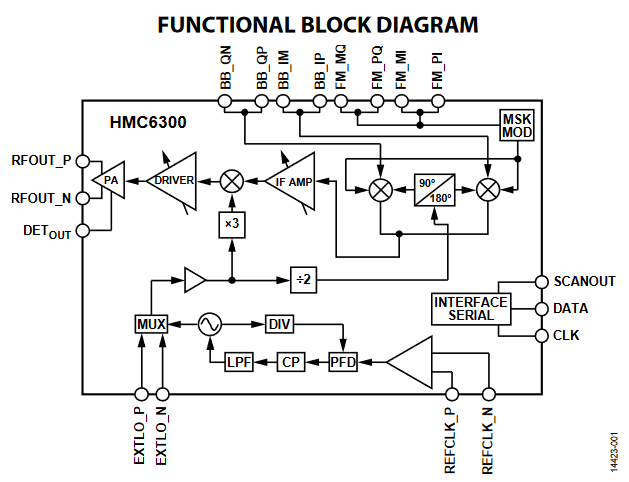
\includegraphics[width = \linewidth - 5cm]{functionalblockdiagram.PNG}
            
            \source{\citeauthor{hmc6300} (\citeyear{hmc6300})}
            \centering
            \label{hmc6300}
        \end{figure}

\subsection{Entrada}

O chip HMC6300 suporta uma frequência de até 900 MHz de largura de banda base. Entretanto, com o nosso objetivo de transmitir um vídeo 4k, teremos que fazer essa modulação em quadratura de 256 QAM para 900 MHz através de uma FPGA.

Primeiramente, para testar se nosso transmissor está funcionando, utilizaremos um gerador de sinais vetoriais ESG, especificamente o E4438C da Agilent\cite{E4438C}, para gerar nossos sinais em quadratura 256 QAM e verificar se está transmitindo os sinais desejados.

Assim, com nosso teste concluído, a placa funcionando, partiremos para a transformação do video em 4k para um sinal em 900MHz 256 QAM através de uma FPGA.

\begin{figure}[htbp]
            \centering
            %\captionsetup{justification=centering}
            \caption{Gerador de sinais vetoriais ESG}
            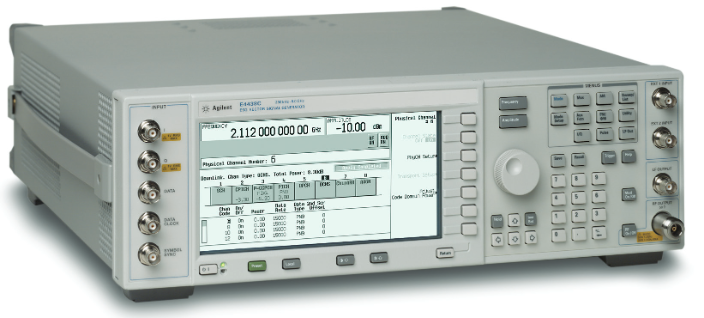
\includegraphics[width = \linewidth - 5cm]{E4438C.PNG}
            
            \source{\citeauthor{E4438C} (\citeyear{E4438C})}
            \centering
            \label{E4438C}
        \end{figure}

\section{Cronograma}

O projeto foi pensado em 4 grandes etapas para serem realizadas em 9 meses. São elas: pesquisa, desenvolvimento do hardware, desenvolvimento do firmware e integração. Na parte de pesquisa é onde procuramos as soluções do mercado, estudos, testes de soluções e nosso planejamento. No desenvolvimento de hardware está centrado principalmente na fabricação, pois como mostrado acima é a parte mais desafiadora desta etapa. Na etapa do desenvolvimento do firmware temos tanto o firmware da configuração quanto o da modulação para a placa. Por último a integração, quando juntamos tudo e fazemos funcionar.

\begin{figure}[htbp]
            \centering
            %\captionsetup{justification=centering}
            \caption{Cronograma}
            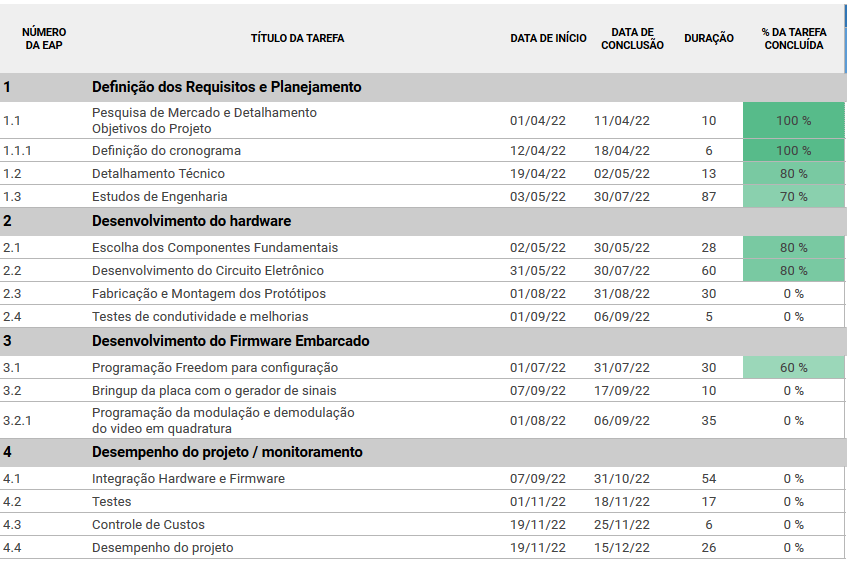
\includegraphics[width = \linewidth - 1cm]{cronograma1.PNG}
            
            \source{De autoria própria}
            \centering
            \label{Cronograma}
        \end{figure}

\begin{figure}[htbp]
            \centering
            %\captionsetup{justification=centering}
            \caption{Cronograma}
            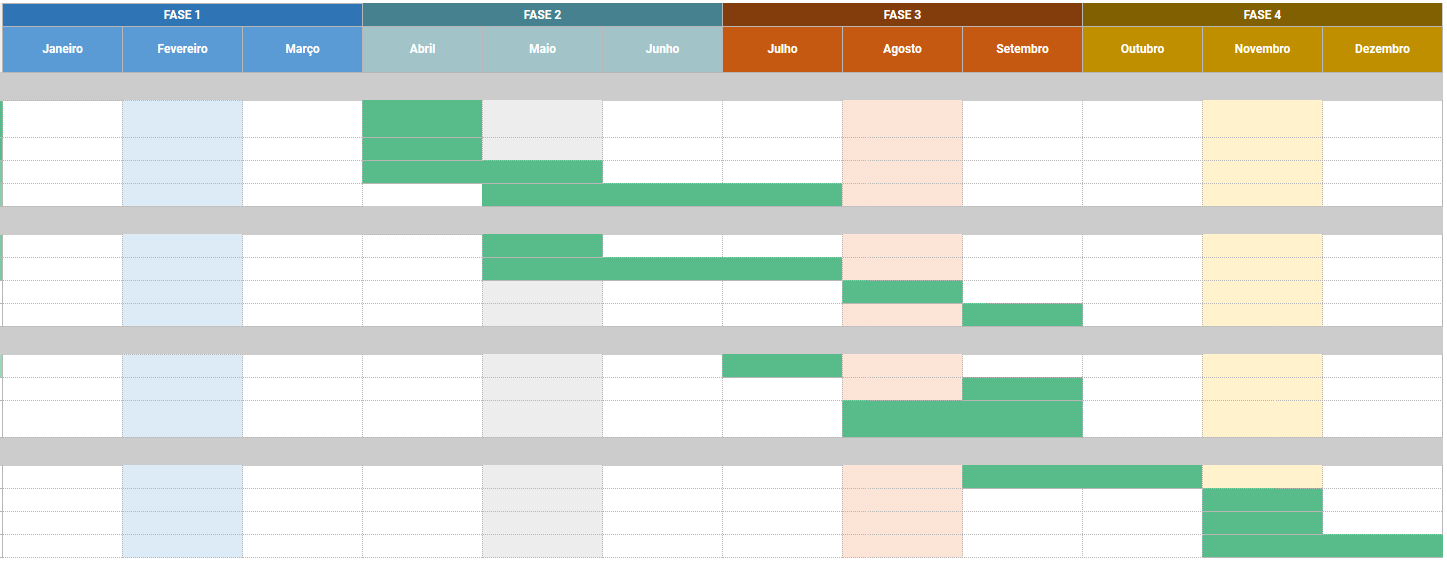
\includegraphics[width = \linewidth - 1cm]{cronograma2.PNG}
            
           \source{De autoria própria}
            \centering
            \label{cronograma2}
        \end{figure}